\section{Vorstellung des Prototypen}
Um die Mehrwerte der Wertschöpfungskette zu verdeutlichen wird ein Prototyp implementiert. Dieser soll den Prozess der Installation, des Updaten und des Nutzen von Softwarepaketen ersichtlich werden lassen und ein technisches Konzept zur Umsetzung der Wertschöpfungskette bereitstellen. Hierzu wird der Absatzprozess abschließend exemplarisch im Kontext von öffentlichen Parkplätzen vorstellt. \textit{Kapitel x\footnote{einfügen}}

Wie in Abbildung \ref{img:basic} zu sehen, umfasst der Prototyp mehrere Teilsysteme. Die Zwei wesentlichen Modulen sind der \textbf{OEM-Server} und das \textbf{Auto} \textit{(Ego-Car)}. Der OEM-Server repräsentiert die Kommunikationsinfrastruktur des Automobilherstellers und ist für das Auto die '\textbf{single source of truth}'. Das Auto wird durch die Zusammensetzung von \textbf{Mensch-Maschine-Schnittstelle} \textit{(HMI)}, \textbf{Car-Control-Unit} \textit{(CCU)} und der \textbf{Carla Simulation} dargestellt.
\begin{figure}[!h]
	\centering
	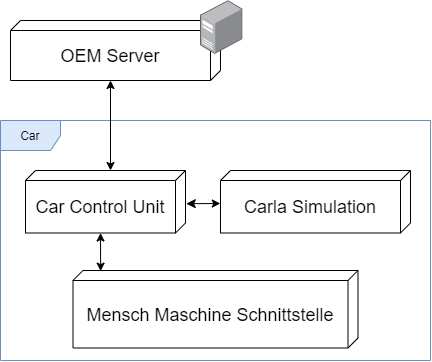
\includegraphics[width=0.5\columnwidth]{pictures/basic.png}
	\label{img:basic}
	\caption{Grundlegende Komponenten}
\end{figure}
Die Carla Simulation beinhaltet die Darstellung eines Autos, dem 'Ego-Car', sowie der Simulation der Autoumwelt. In dieser sind weitere Akteure vorhanden, wie Ampeln, Menschen und andere Autos. Ampeln, Autos und weitere Akteure sollen Nachrichten an das Ego-Car senden können. Diese kommen in der Car Control Unit an. Die CCU stellt eine Kommunikations- und Steuereinheit des Autos dar und ist für die Verwaltung und Nutzung von Software zuständig. Damit eine Software auf Nutzereingaben reagieren kann, wird eine Mensch-Maschine-Schnittstelle in Form einer Android Nutzeroberfläche integriert.\\

Damit der Prototyp genutzt werden kann muss zunächst die Installation der einzelnen Systeme vorgenommen werden. Der PC muss eine gute GPU und Intel CPU verbaut haben. Der OEM-Server und die CCU können mittels der jeweiligen .jar-Datei gestartet werden. Die Mensch Maschine Schnittstelle muss über Android Studio gestartet werden. In der Konfiguration kann der Host der CCU geändert werden, sollte die HMI auf einem separaten gerät laufen. Andernfalls bleibt dies der Lokalhost, da die beiden anderen Systeme auf einen lokalen Port lauschen. Das Starten von Carla erfolgt in Zwei eigenen Schritten. Im ersten wird der Carla \textit{Server} gestartet, welcher die Umgebung von Carla initialisiert. Dies kann auf Windows über die CarlaUE4.exe getan werden. Der zweite Schritt ist das ausführen des Carla-Skripts. Hierdurch wird das Auto in die Welt gesetzt und die Kommunikation mit der CCU initialisiert.\\
Mittels dem 'Szenario Starten'-Knopf in der GUI der CCU  wird der Carla Simulation ein Startimpuls gegeben. Das Auto fährt in der Karte entlang und interagiert mit seiner Umwelt. Das Szenario wird durchgeführt.\\
\begin{center}
	\begin{fminipage}{0.6\textwidth}
		Um den Prototypen zu starten müssen alle Vier Systeme nacheinander gestartet werden:
		\begin{itemize}
			\item[1.] Der OEM-Server \textit{(oem\_server.jar)}
			\item[2.] Die Car Control Unit \textit{(ccu.jar)}
			\item[3.] Die Mensch Maschine Schnittstelle \textit{(via Android Studio)}
			\item[4.] Die Carla Simulation \textit{(über die ccu-gui)}
		\end{itemize}
	\end{fminipage}
\end{center}
\subsection{Gewähltes Szenario}
Das Szenario ist in Zwei Phasen aufgeteilt. Während die nötige Software \textbf{noch nicht} auf dem Auto installiert ist, ist die Rede von \textit{Phase Eins}. Ist die Software installiert, ist von \textit{Phase Zwei} die Rede.\\
In Phase Eins wird die Software installiert oder auf einen neuen Stand upgedatet. Die Installation kann entweder vom Fahrer initiiert werden indem er im Shop die Software kauft und installiert oder sie wird von einem Serviceanbieter initiiert, sobald das Auto in eine 'Registrierungszone' fährt. 

Abbildung \ref{img:communication} zeigt den Ablauf des Szenarioe.
\begin{figure}[!h]
	\hspace{-2cm}
	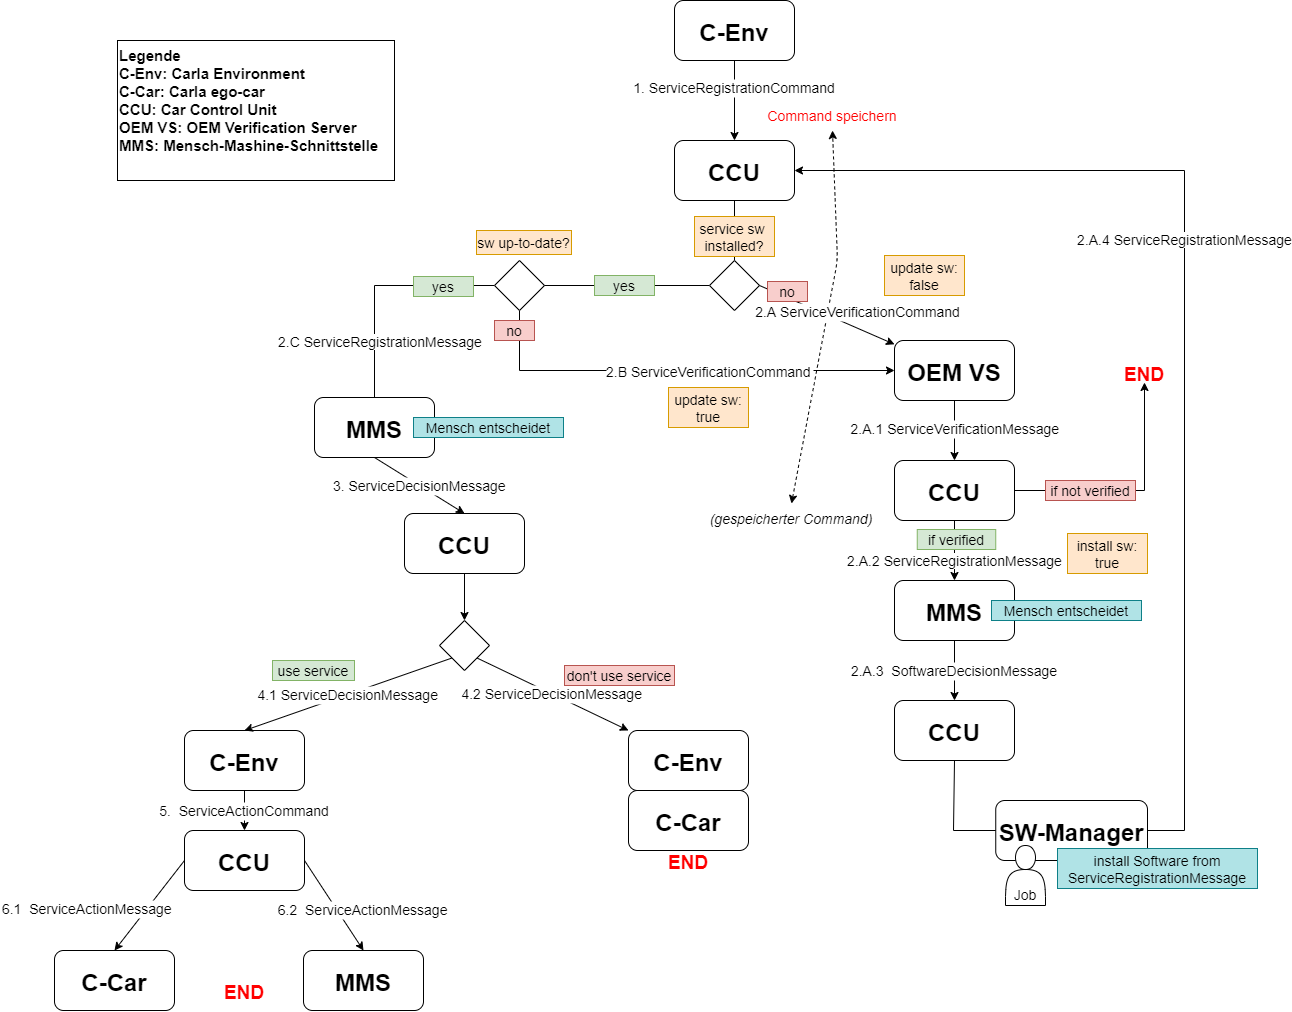
\includegraphics[width=1.2\columnwidth]{pictures/Communication.png}
	\caption{Grundlegende Komponenten}
	\label{img:communication}
\end{figure}

\subsection{Szenario Ablauf}

\subsection{Analyse der Prototypen}
- Mehrwerte aufzählen\\
   Software nutzen auf Autos, welche dem Auto Fahrbefehle gibt.
- Vorteile der gewählten Architektur\\
- Nachteile der gewählten Architektur \& Umsetzung.